\chapter{Graphrepräsentationen}
\label{chap:graph_data}

Das nachfolgende Kapitel basiert, sofern nicht anders vermerkt, auf~\cite{linkeddatatools}.

Eine der Grundlagen der semantischen Daten sowie speziell von semantischen Netzen bilden Graphen. Man spricht in diesem Zusammenhang auch von Graphdatenbanken.

Der Unterschied gegenüber den anonsten gängigen Datenbanken, wie den relationalen oder hierarchischen Datenbanken, liegt vorallem darin, dass die Objekte beliebig verknüpft sein können.

\begin{figure}[htbp]
\centering \rotatebox{0}{\scalebox{0.5}[0.5]{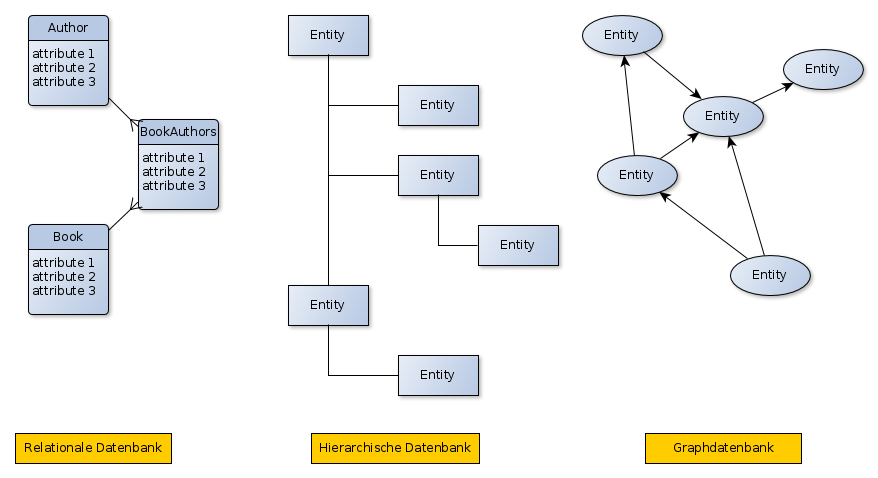
\includegraphics{bilder/datenbanktypen.png}}}
\caption{Darstellung der verschiedenen Datenbanktypen.\label{fig:datenbanktypen}\protect\footnotemark}
\end{figure}
\footnotetext{Eigene Darstellung mittels yEd}

\newpage

Gegeben seien die folgenden Aussagen über Programmiersprachen:
\lstset{caption={Aussagen über Programmiersprachen\protect\footnotemark},captionpos=b}
\lstset{}
\begin{lstlisting}
    C ist eine Programmiersprache.
    C++ ist eine Programmiersprache.
    C++ ist mit C verwandt.
\end{lstlisting}

Verwendet man nun diese Aussagen über Programmiersprachen um daraus eine Graphdatenbank zu erstellen, so ergibt sich folgende Graphdatenbank:
\begin{figure}[htbp]
\centering \rotatebox{0}{\scalebox{0.5}[0.5]{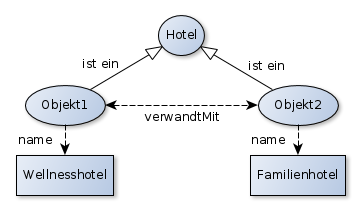
\includegraphics{bilder/programmiersprachen_graph.png}}}
\caption{Aussagen über Programmiersprachen als Graphdatenbank.\label{fig:programmiersprachen_graphdatenbank}\protect\footnotemark}
\end{figure}
\footnotetext{Eigene Darstellung mittels yEd}

In der Graphdatenbank existieren also zwei Objekte, \textit{``Objekt1''} und \textit{``Objekt2''}, mit den Eigenschaften \textit{``ist ein''}, \textit{``verwandtMit''} und \textit{``name''}.

% Graphen.Sven
